\documentclass[11pt]{article}
\usepackage{titling}
\usepackage{multicol}
\usepackage{media9}
\usepackage[english]{babel}
\usepackage[margin=0.6in]{geometry} % Page Dimension
\setlength{\parindent}{0pt}
\usepackage{amsrefs}

%%%%%%%%%%%%%%%%%%%%%%%%%%%%%%%%%%%%%%%%%%
%                PACKAGES                %  
%%%%%%%%%%%%%%%%%%%%%%%%%%%%%%%%%%%%%%%%%%

% Styling Choices
\setlength{\parskip}{\baselineskip}%
\renewcommand{\baselinestretch}{1.2}

% Math
\usepackage{amsmath, amsthm, amssymb}
\usepackage[inline]{asymptote}
\usepackage{enumitem,xcolor}
\usepackage{cancel}
\usepackage{gensymb}
\usepackage{tikz,pgfplots}

% Blind Footnote
\newcommand\blfootnote[1]{%
  \makeatletter{\footnotetext{#1}\makeatother}
}

% Fancy Header
\usepackage{fancyhdr}
\pagestyle{fancy}
\lhead{Kalda Celestial Mechanics}
\rhead{\thepage}

% Coloured Boxes
\usepackage{xcolor}
\definecolor{border}{HTML}{dd1d1d} % 004D4D
\definecolor{hard}{HTML}{ffccb3}
\definecolor{easy}{HTML}{b3e6b3}
\definecolor{normal}{HTML}{f2f2f2}
\definecolor{ans}{HTML}{0060c7}
\usepackage{empheq}
\newcommand*\widefbox[1]{\fbox{\hspace{1em}#1\hspace{1em}}}
\definecolor{claim}{HTML}{BA0030}
\newcommand\boldclaim[1]{\textcolor{claim}{\textbf{#1}}}

% Allows for hyperlinking
\usepackage{hyperref}
\hypersetup{
    colorlinks=true,
    urlcolor=magenta,
    linkcolor=ans,
}

% Syntax: \colorboxed[<color model>]{<color specification>}{<math formula>}
\newcommand*{\colorboxed}{}
\def\colorboxed#1#{%
  \colorboxedAux{#1}%
}
\newcommand*{\colorboxedAux}[3]{%
  % #1: optional argument for color model
  % #2: color specification
  % #3: formula
  \begingroup
    \colorlet{cb@saved}{.}%
    \color#1{#2}%
    \boxed{%
      \color{cb@saved}%
      #3%
    }%
  \endgroup
}

% Setup Gray Question Boxes
\usepackage[breakable,many]{tcolorbox}
\newtcolorbox[auto counter]{solution}[1]{
    enhanced, breakable,
    arc=0pt,
    % colback=default, % Background color
    colframe=white, % Border Color
    coltitle=black, % Title Color
    fonttitle=\bfseries,
    title=\fcolorbox{border}{#1}{\textcolor{border}{pr} \bfseries \textcolor{border}{\thetcbcounter}.},
    attach title to upper,
    after title={\ },
    segmentation style={dashed, gray},
}

% Setup Gray Solution Boxes
\usepackage[breakable,many]{tcolorbox}
\newtcolorbox[auto counter]{answer}[1]{
    enhanced, breakable,
    arc=0pt,
    % colback=default, % Background color
    colframe=white, % Border Color
    coltitle=black, % Title Color
    fonttitle=\bfseries,
    title=\fcolorbox{ans}{#1}{\hyperlink{P\thetcbcounter}{\textcolor{ans}{sol} \bfseries \textcolor{ans}{\thetcbcounter}}.},
    attach title to upper,
    after title={\ },
    segmentation style={dashed, gray},
}

% Title and front page
\title{Translation of Celestial Mechanics Handout by Mikhel Kree}
% Author
\author{\textsc{Daniel Yang, Kushal Thaman, Ashmit Dutta}}

\begin{document}
\begin{titlepage}
    \begin{center}
        \vspace*{1cm}
 
        \Huge
        \textbf{Translation of “Kepleri Seadused Ja Muu Taevamehaanika”}
 
        \vspace{0.5cm}
        \LARGE
        Edition 0.7.0
        
        \vspace{0.5cm}
        Daniel Yang, Kushal Thaman, Ashmit Dutta
        
        \begin{center}
            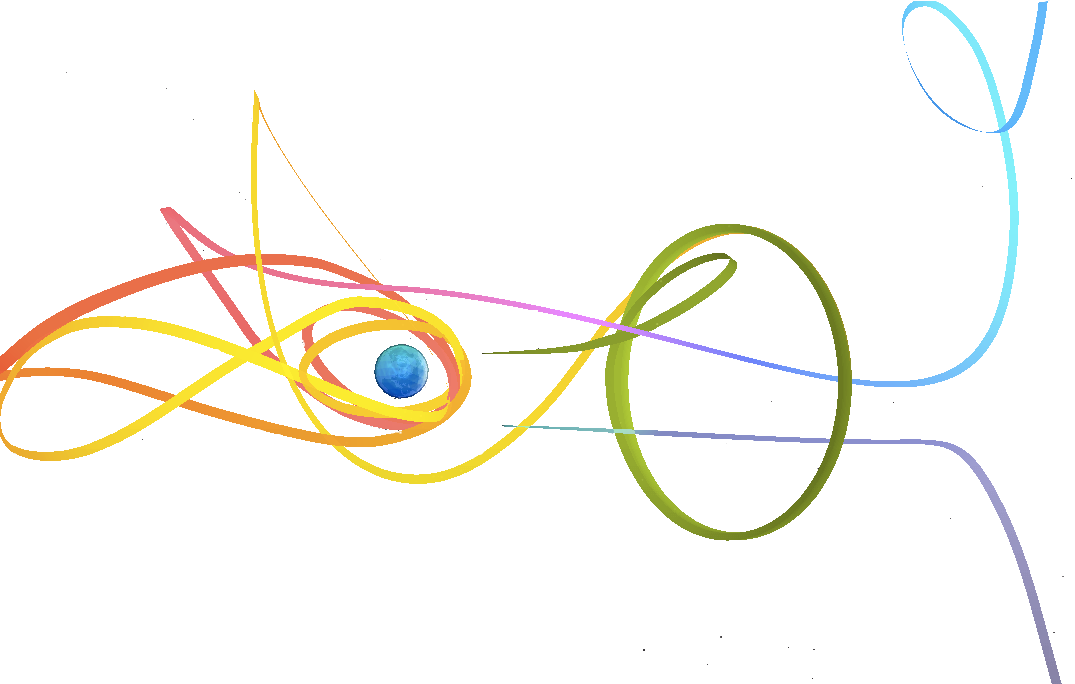
\includegraphics[width=0.95\linewidth]{Images/halo_orbit_title.png}
        \end{center}
        \normalsize
        ~\cite{haloSE}

        \vspace{1mm}
        \Large
        Edited by: QiLin Xue
        
        \Large
        Updated
        \today
 
    \end{center}
\end{titlepage}
\newpage
%%%%%%%%%%%
% Preface %
%%%%%%%%%%%
\section*{Preface}
\vspace{-5mm}
\indent Jaan Kalda's \href{https://www.ioc.ee/~kalda/ipho/}{handouts} are beloved by physics students both in for a quick challenge, to students preparing for international Olympiads. The current \href{https://www.ioc.ee/~kalda/ipho/kepler.pdf}{celestial mechanics} handout (written by Mihkel Kree, ver 0.7) is, unfortunately for people not fluent in Estonian, fully in Estonian~\cite{kaldakepler}. Here, we have attempted to translate the entire handout.

\subsection*{Contact Us}
\vspace{-5mm}
Because none of the authors of this document actually know Estonian, we used a combination of Google Translate and observing similarities between the handout and other English-language documents. As a result, some of the translations here are likely wrong or a misinterpretation of the original text. If you do find any mistakes, or know the source of a specific problem, then please contact us at \href{mailto:hello@physoly.tech}{hello@physoly.tech}. The most current and updated version of this document can be found on our website \href{https://physoly.tech/}{physoly.tech}.

Please feel free to contact us at the same email if you are confused on a question. Chances are that many others will have the same question as you.

\newpage
\vspace{-5mm}
\section{Introduction}
\vspace{-5mm}
In this handout we take a look at the basic properties of an ellipse and the important features of an ellipse in relation to gravity. We derive all three of Kepler's laws with some effort based on known conservation laws. We'll also take a look at some tricks in solving planetary motion problem using our main tools of (as expected) conservation of energy and momentum. Among other things, we prove that the total energy of a planet does not depend on the shape of its orbit, but only its semi-major axis. The solutions to the problems are located in the last chapter.
\vspace{-5mm}
\section{Ellipses}
\vspace{-5mm}
An ellipse is essentially a stretched circle. For example, consider a circle of radius $r=b$ and stretch it in the $x$-axis by a coefficient of expansion $k=a/b>1$. We now have an ellipse with semi-minor axis $b$ and semi-major axis $a$. The area of the ellipse is, of course, $S=\pi ab$.
\begin{center}
    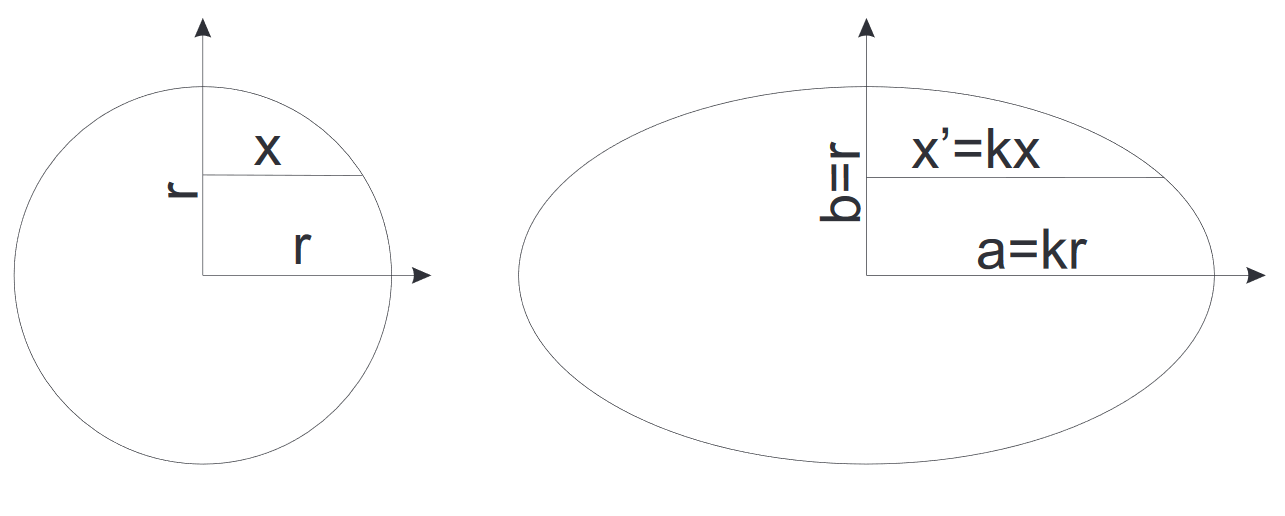
\includegraphics[width=0.8\textwidth]{Images/CM1.png}
    
    Figure 1: Stretching a circle, we get an ellipse
\end{center}
Traditionally, an ellipse is defined by two foci and a semi-major axis, where the sum of the distances of each point on the ellipse to the foci is equal to twice the semi-major axis: $r_1+r_2=2a$. Sometimes it is also necessary to focus on the distance $c$ to the center of the ellipse. In fact, the eccentricity of an ellipse is defined as $e=c/a<1$. It is easy to see that $a^2=b^2+c^2$.

A tangent drawn at any point of an ellipse is at the same angle to the lines connecting that point with the two foci of the ellipse. (This ``reflection property" explains why in an elliptical space, a sound source located at one focus is heard very clearly at the other focus). Since it is sometimes necessary to use the equations of an ellipse in problems, we will present them here. If the center of an ellipse is at the origin, it is defined by the equations
\begin{align*}
    y&=b\sin\phi \\
    x&=a\cos\phi \\
    1&=\left(\dfrac{x}{a}\right)^2+\left(\dfrac{y}{b}\right)^2
\end{align*}
% $$y=b\sin\phi,\;\;\;\;x=a\cos\phi,\;\;\;\;\text{or}\;\;\;\;\left(\dfrac{x}{a}\right)^2+\left(\dfrac{y}{b}\right)^2=1.$$
\begin{center}
    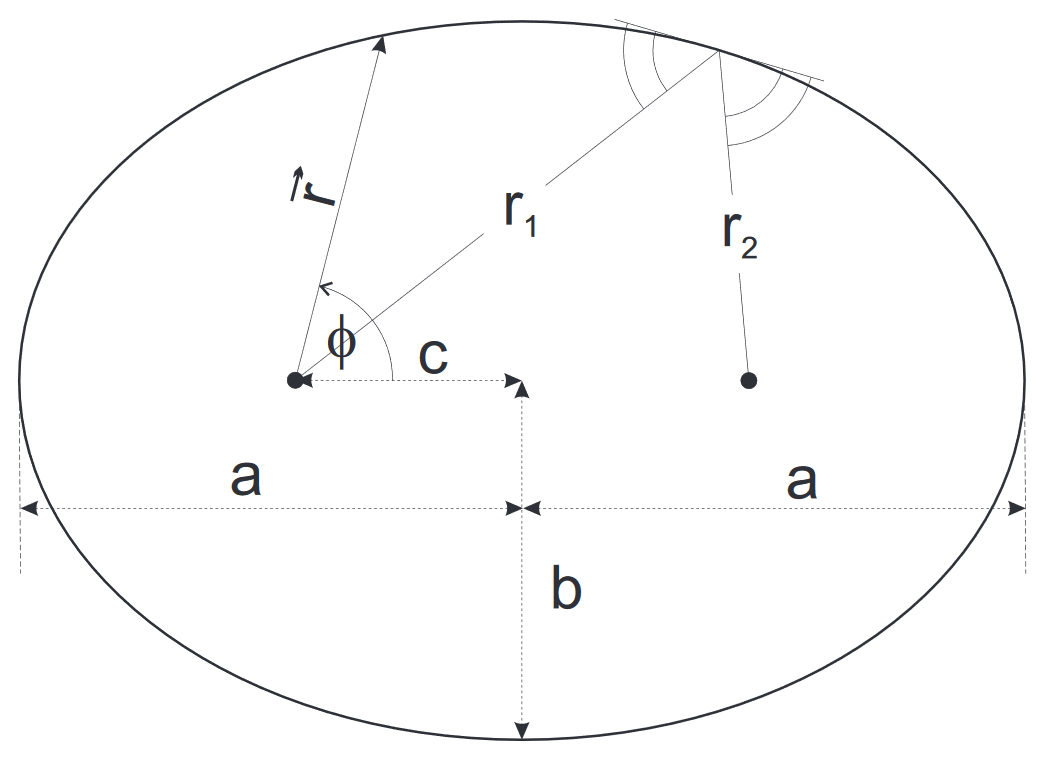
\includegraphics[width=0.6\textwidth]{Images/CM2.png}
    
    Figure 2: The figure above shows the semi-major and semi-minor axes of an ellipse as well as some of its properties and the definition of the polar coordinates used.
\end{center} % the figure may be wrong: I don't think that's what $\phi$ is supposed to be
The following is an equation of an ellipse in polar coordinates with respect to the foci:
$$r=\dfrac{a(1-e^2)}{1-e\cos^2\theta}.$$
\vspace{-10mm}
\section{Gravitational Fields}
\vspace{-5mm}
The force between two point masses is known to be
\begin{equation}
    F=\dfrac{GMm}{r^2}.
\end{equation}
We define the gravitational potential energy of an object (negative) to be the work per unit mass that would be needed to move an object from infinity to some location in space.
\begin{equation}
    E_p=-\dfrac{GMm}{r}.
\end{equation}
Additionally, the gravitational field strength is related to the potential energy by the formula $\displaystyle F=-\frac{dE}{dr}$.
\hypertarget{P1}{}
\begin{solution}{normal}
Determine the orbital period of an object that orbits in a circular path of radius $R$ around the Earth if the radius of the Earth is $R_M$.
\end{solution}
One type of problem deals with the mass distribution within a planet. Consider a spherical object of radius $R$ and its gravitational field at radius $r\leq R$. If the mass distribution is spherically symmetric, then then gravitational field of points located at $r\leq x\leq R$ from the center of the object cancel each other out. \textit{Note:} This is also known as the shell theorem. For for following problems, assume that all objects are of uniform density.
\hypertarget{P2}{}
\begin{solution}{normal}
Find the time it takes to ``fall" through a straight hole passing through the center of the Earth. \textit{Hint:} The position dependence of acceleration should be similar to that of a harmonic oscillator $a=-\omega^2x$. Compare this with the time it takes or orbit Earth at ground level. How would the result change if the hole did not pass through the center of the Earth?
\end{solution}
\hypertarget{P3}{}
\begin{solution}{normal}
Prove that the gravitation field is constant in a spherical cavity inside a planet.
\end{solution}

\vspace{-5mm}
\section{Kepler's Laws}
\vspace{-5mm}
We present Kepler's Laws in order of simplicity.

\textbf{Kepler's Second Law.} Prove that the angular momentum $\vec{L}=\vec{r}\times\vec{p}$ (where the star is at the origin) does not change over time and relate it to the rate at which the line joining a planet and a star sweeps out area.

\textbf{Solution.} If we consider the angular momentum with respect to an axis perpendicular to the plane and passing through the star, the we notice that the momentum cannot change as the only force acting on the planet is directed towards the reference axis. Therefore:
$$\dfrac{d\vec{L}}{dt}=\vec{M}=0,\;\;\;\;\vec{L}=\text{const.}$$
We can reach the same result algebraically using the chain rule:
$$\dfrac{d\vec{L}}{dt}=\dfrac{d\vec{r}}{dt}\times\vec{p}+\vec{r}\times\dfrac{d\vec{p}}{dt}=\vec{v}\times\vec{p}+\vec{r}\times\vec{F}=0,$$
since velocity and momentum are directed in the same direction, as well as the radius vector and force. The cross product of vectors in the same direction is known to be zero.

We then find the area covered by the radius vector in a small time interval $\Delta t$. The area swept through is a triangle with height equal to the radius and base equal to the distance travelled by the planet during this time:
$$\Delta S=\dfrac{1}{2}rv_\bot\Delta t=\dfrac{L}{2m}\Delta t,$$
where we substituted in the expression for angular momentum. Clearly, the area of this region does not depends on the radius of orbit, but solely on the time period. Therefore, the radius vector sweeps through equal areas in equal times.

\textbf{Kepler's First Law.} Show that the orbit of a planet is elliptical, knowing the equation of an ellipse in polar coordinates is given by: $r=A/(1+e\cos\theta)$. \textit{Hint:} First make sure that $\displaystyle \frac{d}{dt}(\vec{v}\times\vec{L})=GMm\frac{d\vec{e_r}}{dt}$, where $\vec{e_r}$ is the radial unit vector.

\textbf{Solution.} This solution is mathematically difficult, so it is fine to simply follow along the solution. Let's start from the hint by denoting the mass of the star $M$, the mass of the planet $m$, and the radial unit vector $\vec{e_r}$:
$$\dfrac{d}{dt}(\vec{v}\times\vec{L})=\dfrac{d\vec{v}}{dt}\times\vec{L}+\vec{v}\times\dfrac{d\vec{L}}{dt}=\dfrac{d\vec{v}}{dt}\times\vec{L}=\vec{a}\times\vec{L}=\dfrac{1}{m}\vec{F}\times\vec{L}=-\dfrac{GM}{r^2}\vec{e_r}\times\vec{L}.$$
In the following equations, note that $r$ denotes the modulus of the radius vector and $\vec{r}$ is the vector itself:
$$\vec{r}=r\vec{e_r},\;\;\;\;\vec{v}=\dfrac{d(r\vec{e_r})}{dt}=\dfrac{dr}{dt}\vec{e_r}+r\dfrac{d\vec{r_e}}{dt},$$
$$\vec{L}=\vec{r}\times\vec{p}=m\vec{r}\times\left(\dfrac{dr}{dt}\vec{e_r}+r\dfrac{d\vec{e_r}}{dt}\right)=mr^2\left(\vec{e_r}\times\dfrac{d\vec{e_r}}{dt}\right),$$
Since $\vec{r}$ and $\vec{e}_r$ are parallel, the vector product disappears. Next, we use the rule for converting the vector products to scalar products $\vec{a} \times (\vec{b} \times \vec{c}) = \vec{b}(\vec{a}\vec{c})-\vec{c}(\vec{a}\vec{b})$
$$\frac{d}{d}(\vec{v}\times\vec{L})=-\frac{Gm}{r^2}\vec{e}_r \times \vec{L} = -GMm\vec{e}_r \times \left(\vec{e}_r\times \frac{d \vec{e}_r}{dt}\right)$$
$$= -GMm\vec{e}_r \left(\vec{e}_r \frac{d \vec{e}_r}{dt}\right)+GMm\frac{d \vec{e}_r}{dt}(\vec{e}_r \vec{e}_r) = GMm\frac{d \vec{e}_r}{dt}$$
as $\vec{e}_r$ and $\displaystyle\frac{d\vec{e}_r}{dt}$ are perpendicular to teach other and the square of $\vec{e}_r$ is one. Before differentiation, we have the equation
\begin{equation}\label{eq:3}
    \vec{v}\times\vec{L}=GMm\vec{e}_r+\vec{C},
\end{equation}
where $\vec{C}$ is a constant vector. Equation (3) is also worth remembering, as we will return to it later in connection to a problem. Finally, to complete our proof, we can see that
$$L^2=\vec{L}\left(\vec{r}\times m\vec{v}\right)=m\vec{r}\left(\vec{v}\times\vec{L}\right)=mr\left(GMm+C\cos(\theta)\right),$$
where we have used the formula $\vec{a}(\vec{b}\times\vec{c})=\vec{b}(\vec{c}\times\vec{a})$ and where $\theta$ denotes the angle between the vectors $\vec{r}$ and $\vec{C}$. Finding $r$ from the last expression, we get that
$$r=\dfrac{\frac{L^2}{GMm^2}}{1+\frac{C}{GMm}\cos\theta}.$$
From this, we have shown that a planet (of negligible mass compared to its star) orbiting a star moves along an elliptical orbit, one of whose foci is at the star.

\textbf{Kepler's Third Law.} Show that the orbital period of a planet around a star of mass $M$ in an orbit with semi-major axis $a$ is given by
\begin{equation}
    T^2=\dfrac{(2\pi)^2a^3}{GM}.
\end{equation}
\textit{Additional problem:} Show that in a binary star system the stars move in elliptical orbits one of whose foci (for each orbit) is at the center of mass of the system and show that the orbital period of the system is given by
$$T^2=\dfrac{(2\pi)^2\left(a_1+a_2\right)^2}{G\left(M_1+M_2\right)}$$

\textbf{Solution.}  Let's first look at how to relate speed and acceleration (or gravitational forces). Let the body move in a circle for an infinitely short time so that the displacement in the horizontal direction (see figure) would be $x$ and $h$ in the vertical direction.

\begin{center}
    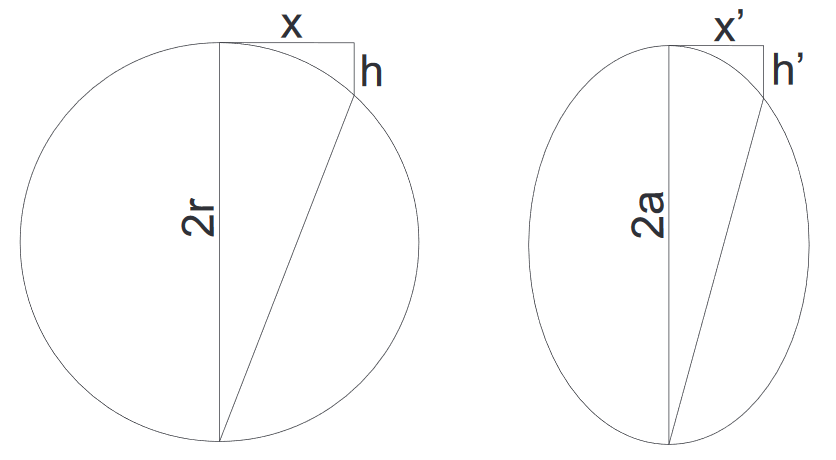
\includegraphics[width=0.6\linewidth]{Images/CM3.png}
\end{center}

From the equality of boundary angles we get similar triangles
\[\frac{h}{x} = \frac{x}{2r - h}\approx \frac{x}{2r},\hspace{10pt} h = \frac{x^2}{2r}.\]
Let this movement take place during the period $\Delta t$. Denoting the horizontal velocity $v$ and the vertical acceleration $F/m$, we get:
\[x = v\Delta t, \hspace{15pt} h = \frac{\frac{F}{m}(\Delta t)^2}{2} = \frac{v^2(\Delta t)^2}{2r}, \hspace{15pt} \frac{F}{m} = \frac{v^2}{r}.\]
So we have found the acceleration in circular motion. Now move the object to the perigee of its elliptical orbit (closest point to a focus). The corresponding displacements are denoted by $x'$ and $h'$ (see figure). If we compress the ellipse in the direction of the semi-major axis by a coefficient $k = a / b$, we would get a circle with radius $r = b$. Doing that and combining it with our earlier result, we can see that:
\[\frac{h'}{k} = \frac{x'^2}{2b}, \hspace{15pt} h' = \frac{x'^2 a}{2b^2}, \hspace{15pt} \frac{F}{m} = \frac{v^2 a}{b^2},\]
where we have switched to acceleration and speed. The distance of the perigee from the focus is $a - c$, hence
\[F = \frac{GMm}{(a-c)^2}, \hspace{15pt} v^2 = \frac{Fb^2}{ma} = \frac{GMmb^2}{ma(a-c)^2} = \frac{GM(a^2 - c^2)}{a(a - c)^2} = \frac{GM (a + c)}{a(a - c)},\]
where we proceeded from the relation $a^2 = b^2 + c^2$. To determine the orbital period, we use Kepler's Second law (i.e. the time-area equality):
\[\frac{T}{S} = \frac{\Delta t}{\Delta S}, \hspace{15pt} T = \pi ab\frac{\Delta t}{\frac{(a - c)v\Delta t}{2}} = \frac{2\pi ab}{(a - c)v},\]
where the area of the ellipse is $S = \pi ab$ and the area of the smaller section was from an isosceles triangle with base $v\Delta t$ and height $a-c$. Since we already have an expression for $v^2$, we can find that
\[T^2 = \frac{(2\pi)^2a^2b^2}{(a - c)^2v^2} = \frac{(2\pi)^2a^2b^2a(a-c)}{(a-c)^2GM(a + c} =  \frac{(2\pi)^2a^3b^2}{GM(a^2-c^2)}= \frac{(2\pi)^2a^3}{GM},\]
proving Kepler's Third Law (the square of the period is proportional to the cube of the semi-major axis). Note that the constant of proportionality is given by
$$\dfrac{T^2}{a^3}=\dfrac{4\pi^2}{GM}.$$

\newpage
\vspace{-5mm}
\section{Energy}
\vspace{-5mm}
\hypertarget{P4}{}
\begin{solution}{normal}
Derive the expression for total energy (kinetic plus potential):
\begin{equation}\label{eq:5}
    E=-\dfrac{GMm}{2a}.
\end{equation}
\end{solution}
If the total energy is negative, then the object is unable to escape the gravitational field of the star to the point at infinity since infinitely far away, the potential energy is zero and the total energy would be equal to the kinetic energy, which cannot be negative. Sometimes problems give an object enough speed to escape the gravitational field, in which case the total energy would be positive.

\vspace{-5mm}
\section{Problems}
\vspace{-5mm}
\hypertarget{P5}{}
\begin{solution}{normal}
An object is thrown vertically from the ground and reaches a distance $R=R_M$ above the surface of the Earth before returning. If $R_M$ is the radius of the earth, determine the time of flight of the object.
\end{solution}
\hypertarget{P6}{}
\begin{solution}{normal}
An object is sent into orbit via a two-stage process. First, the object has a velocity $v_1$ at the ground, and at the apogee of its orbit its velocity is increased to $v_2=v+\Delta v$ so that the object is now in a circular orbit at radius $R$. If the radius of the Earth is $R_M$, determine $v_1$ and $\Delta v$.
\end{solution}
\hypertarget{P7}{}
\begin{solution}{normal}
An object moving in a circular orbit with radius $R$ is given extra radial velocity. How large must this velocity be in order for the object to escape Earth's orbit? The radius of the earth is $R_M$. \textit{Hint:} What must be the total energy of the object to get it out of orbit?
\end{solution}
\hypertarget{P8}{}
\begin{solution}{normal}
An explosion takes place near a star, causing many small objects to fly outwards with speed $v$. The objects begin to move in elliptical orbits, with one of the foci at the star. Determine the locus (set of possible positions) of the second focus.
\end{solution}
\hypertarget{P9}{}
\begin{solution}{normal}
Let us consider the gravitational compression of an interstellar gas cloud. Assume that the gas has density $\rho=10^{-15}\;\text{kg}/\text{m}^3$ and fills a spherical space. Assume that the temperature is so low that the initial velocity of the gas particles is zero. How long does it take for the gas cloud to shrink?
\end{solution}
\hypertarget{P10}{}
\begin{solution}{normal}
From a point at infinity, an object approaches a star and then moves off back to infinity. Drawing the two asymptotes to the trajectory of the object, they meet at an angle $\phi<90\degree$ and have minimum distance $b$ and $b'$ from the star. Determine the relationship between $b$ and $b'$ and find an expression for the angle $\phi$. \textit{Hint:} Statement \ref{eq:3} may be useful.
\begin{center}
    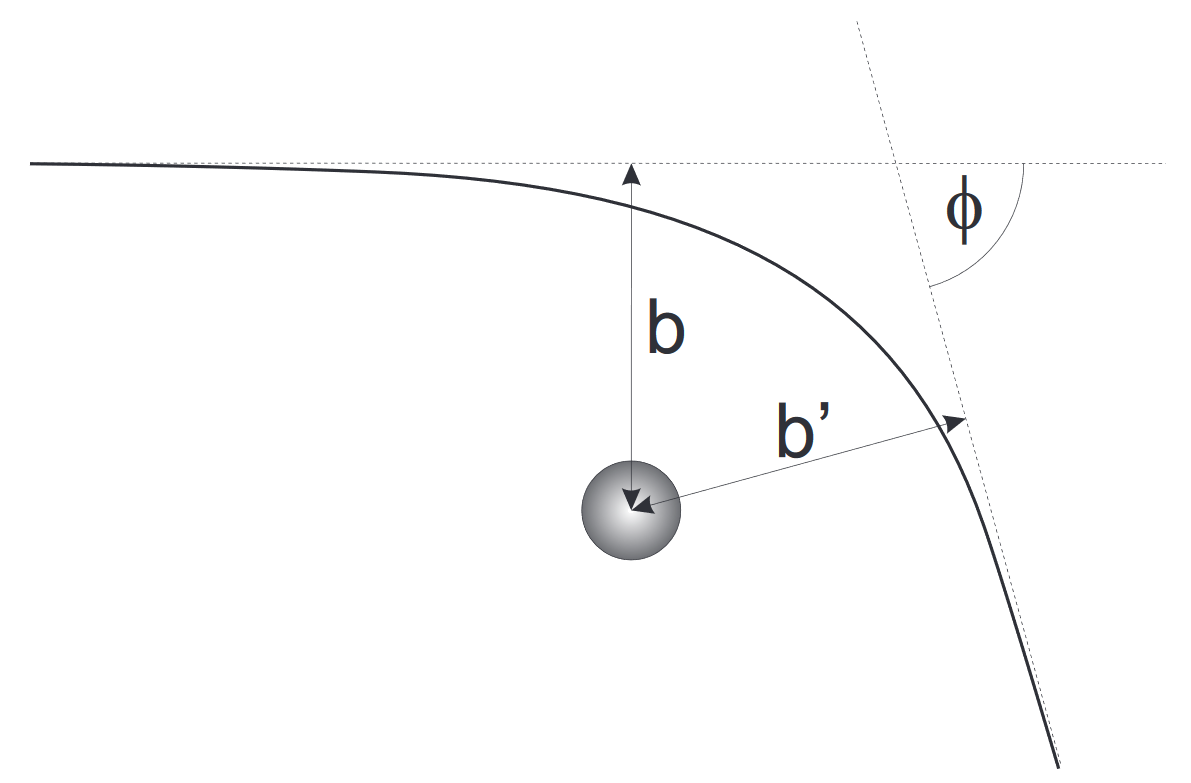
\includegraphics[width=0.6\linewidth]{Images/CM4.png}
\end{center}
\end{solution}
\vspace{-4mm}
\subsection{More Problems}
\vspace{-2mm}
Both Estonian and international olympiads sometimes have problems related to celestial mechanics (abbeviations: EFO - Estonian Physics Olympiads, ES - Estonian-Finnish Physics Olympiad, IPhO - International Physics Olympiad):
\begin{itemize}
    \item EFO 2001, \href{https://www.teaduskool.ut.ee/sites/default/files/teaduskool/olympiaad/eesti/efo_01_02_lv_ylesanded_g_ee.pdf}{Problem 8 - Binary Star System}
    \item ES 2005, \href{https://www.ioc.ee/~kalda/ipho/es/E_S_2005_e.pdf}{Problem 3 - Ballistic Rocket}
    \item ES 2004, \href{https://www.ioc.ee/~kalda/ipho/E_S2.pdf}{Problem 2 - Planets}
    \item IPhO 2005, \href{https://www.ioc.ee/~kree/students/iphoTable/files/ipho/2005_Spain_p1.pdf}{Problem 1 - An Ill Fated Satellite}
    \item IPhO 2001, \href{https://www.ioc.ee/~kree/students/iphoTable/files/ipho/2001_Turkey_p2.pdf}{Problem 2 - (Another) Binary Star System}
    \item IPhO 1999, \href{https://www.ioc.ee/~kree/students/iphoTable/files/ipho/1999_Italy_p3.pdf}{Problem 3 - A Space Probe to Jupiter}
    \item IPhO 1996, \href{https://www.ioc.ee/~kree/students/iphoTable/files/ipho/1996_Norway_p3.pdf}{Problem 3 - Moon and Tides}
\end{itemize}
Translation of EFO 2001 Problem 8: - Binary Star System
\hypertarget{P11}{}
\begin{solution}{normal}
The masses of two stars in a binary star system are $M_1$ and $M_2$. Their initial values are $M_{1_0}=1.5M_{\odot}$ and $M_{2_0}=3M_{\odot}$ (where $M_\odot$ denotes the mass of the Sun) and the system rotates around its center of mass with orbital period $T_0=10\text{ years}$. Mass continually flows from the first star to the second star at a rate of $\mu=10^{-7}\;M_\odot/\text{yr}$. (a) Prove that during this process the quantity $M_1M_2va$ stays constant, where $v$ is the relative velocity of the stars and $a$ is the distance between them. (b) Prove that the quantity $v^2a$ remains constant. (c) At what rate does the orbital period of the stars change? \textit{Note:} The angular momentum of the isolated system remains constant, i.e. $M_1v_1a_1+M_2v_2a_2=\text{const}$, where $a_1$, $a_2$ are the distances from the stars to their center of mass and $v_1$, $v_2$ are their velocities.
\end{solution}
\vspace{-5mm}
\section{Solutions}
\begin{answer}{normal} % sol 1
To move in a circular orbit, the acceleration must be provided by the gravitational force $$a = \frac{v^2}{R} , a= \frac{GM}{R^2}, v = \sqrt{\frac{GM}{R}}$$ The orbital time period, or the time taken to go around a circle is $$T = \frac{2\pi R}{v} = 2\pi\sqrt{\frac{R^3}{GM}}$$
\end{answer}

\begin{answer}{normal} % sol 2
We solve the problem in general, where the minimum distance from then tunnel to the center of the Earth is $b$. Let the object be located at some distance $x$ from the midpoint of the tunnel and a distance $r$ from the center of the Earth (see the figure below). By the shell theorem, the effective part of the Earth acting upon the object lies within a sphere of radius $r$ from the center of the Earth:
$$F=-\dfrac{GM'm}{r^2},\;\;\;\text{where}\;\;\;M'=\dfrac{4}{3}\pi r^3\rho.$$
However, we are interested only in the component of the force acting along the tunnel:
$$F_\parallel=F\cos\alpha=F\dfrac{x}{r}=-\dfrac{GM'mx}{r^3}=-G\dfrac{4}{3}\pi\rho mx.$$
Expressing $\rho$ as a function of $M$ and $R$, we obtain:
$$\rho=\dfrac{M}{\frac{4}{3}\pi R^3},\;\;\;a=-\dfrac{GM}{R^3}x.$$
\begin{center}
    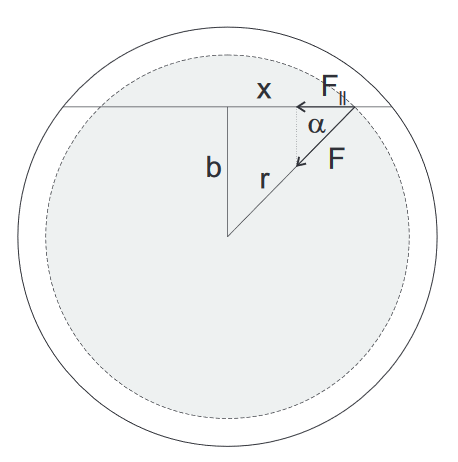
\includegraphics[width=0.35\linewidth]{Images/CM5.png}
\end{center}
This equation is simple harmonic motion and has solution
$$x=\cos(\omega t),\;\;\;a=\dfrac{d^2x}{dt^2}=-\omega^2\cos(\omega t)=-\omega^2x,\;\;\;\text{therefore}$$
$$\omega^2=\dfrac{GM}{R^3},\;\;\;T=2\pi\sqrt{\dfrac{R^3}{GM}}.$$
\end{answer}

\begin{answer}{normal} % sol 3
We can imagine the cavity as a superposition of a large sphere of density $\rho$ and a smaller sphere of radius $-\rho$, where the smaller sphere is completely contained within the larger sphere. From here we get two accelerations (see the figure below):
$$\vec{a}_1=-GM_1\dfrac{\vec{r}_1}{|r_1|^3}\;\;\;\text{and}\;\;\;\vec{a}_2=-GM_2\dfrac{\vec{r}_2}{|r_2|^3}.$$
\begin{center}
    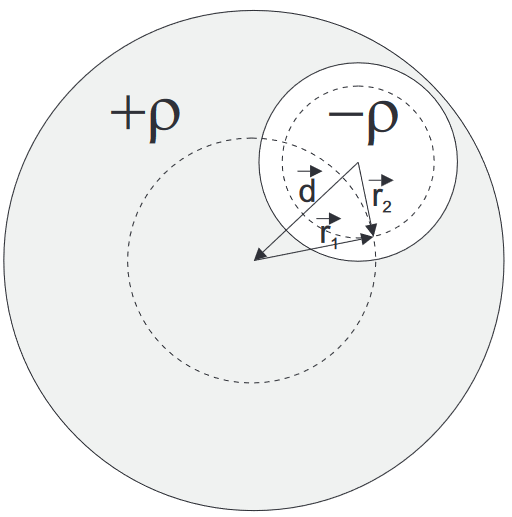
\includegraphics[width=0.4\linewidth]{Images/CM6.png}
\end{center}
Note that the denominator is of degree three since the numerator is a vector.
$$M_1=\dfrac{4}{3}\pi r_1^3\rho,\;\;\;M_2=-\dfrac{4}{3}\pi r_2^3\rho,\;\;\;\text{which gives total acceleration}$$
$$\vec{a}=\vec{a}_1+\vec{a}_2=G\dfrac{4}{3}\pi\rho\left(-\vec{r}_1+\vec{r}_2\right)=\dfrac{4}{3}G\pi\rho\vec{d}.$$
As a result, the gravitational field is the same at every point in the cavity and is in the direction of the line connecting the centers of the spheres.
\end{answer}

\begin{answer}{normal} % sol 4
Since the total energy of the object in orbit does not change, we write energy expressions at the apogee and perigee of the object's orbit:
$$E=\dfrac{mv_1^2}{2}-\dfrac{GMm}{r_1},\;\;\;E=\dfrac{mv_2^2}{2}-\dfrac{GMm}{r_2}.$$
We consider the conservation of angular momentum: $r_1v_1=r_2v_2$. We multiply the first (energy) equation by $r_1^2$ and the second by $r_2^2$ and subtract, noting that $r_1=a-c$ and $r_2=a+c$:
$$E\left(r_1^2-r_2^2\right)=-GMm(r_1-r_2),$$
$$E=-GMm\dfrac{r_1-r_2}{r_1^2-r_2^2}=-\dfrac{GMm}{r_1+r_2}=-\dfrac{GMm}{2a}.$$
\end{answer}

\begin{answer}{normal} % sol 5
The flight path of the object is along an infinitely narrow ellipse with semi-major axis $R/2$ (one focus is at the center of the earth and the other is at the tip of the trajectory of the object). The period of orbit depends solely on the semi-major axis (by Kepler's third law), which we found in Problem 1. Furthermore, the area swept through by the radius vector is proportional to the time of flight. Here, the radius vector covers an area consisting of half the area of an ellipse and an isosceles triangle (of base $2b$ and height $a$):
$$\dfrac{\tau}{S'}=\dfrac{T_0}{S_0},\;\;\;\text{where}\;\;\;S_0=\pi ab\;\;\;\text{and}\;\;\;S'=\dfrac{1}{2}\pi ab+ba.$$
So we have that
$$\tau=\dfrac{\frac{1}{2}\pi+1}{\pi}T_0=\dfrac{\frac{1}{2}\pi+1}{\pi}\cdot2\pi\sqrt{\dfrac{a^3}{GM}}=\left(\dfrac{\pi}{2}+1\right)\sqrt{\dfrac{R^3}{2GM}}.$$
More generally, if the object were to reach a height $R\neq R_M$ above the surface of the Earth, we have that $a=(R_M+R)/2$ and
$$S'=\pi ab-\arccos\left(\dfrac{a-R_M}{a}\right)ab+\dfrac{bR_M}{a}\sqrt{R_M(2a-R_M)}$$
$$\tau =\dfrac{\pi-\arccos\left(\frac{a-R_M}{a}\right)+\frac{R_M}{a^2}\sqrt{R_M(2a-R_M)}}{\pi}T_0$$
$$\tau=\left(2\pi-2\arccos\left(\dfrac{a-R_M}{a}\right)ab+\dfrac{2R_M}{a^2}\sqrt{R_M(2a-R_M)}\right)\sqrt{\dfrac{a^3}{GM}}\text{, where }a=\dfrac{R_M+R}{2}$$
\end{answer}

\begin{answer}{normal} % sol 6
Initially, the object moves along an elliptical orbit with semi-major axis $R+R_M$. Knowing the total energy and the potential energy of the object we can get the initial kinetic energy:
$$E=-\dfrac{GMm}{R_M+R},\;\;\;E_k=E-E_p=GMm\left(\dfrac{1}{R_M}-\dfrac{1}{R_M+R}\right),\;\;\;v=\sqrt{\dfrac{2GMR}{R_M(R+R_M)}}.$$
To find the increase in velocity, we determine the velocity at the apogee of the orbit:
$$v_a=\sqrt{\dfrac{2GMR_M}{R(R+R_M)}},\;\;\;v_2=\sqrt{\dfrac{GM}{R}},\;\;\;\Delta v=v_2-v_a$$
$$\Delta v=\sqrt{\dfrac{GM}{R}}\left(1-\sqrt{\dfrac{2R_M}{R+R_M}}\right)$$
\end{answer}

\begin{answer}{normal} % sol 7
A body moving in a circular orbit has velocity perpendicular to the radius and potential energy:
$$v_\bot=\sqrt{\dfrac{GM}{R}}\;\;\;\text{and}\;\;\;E_p=-\dfrac{GMm}{R}.$$
The radial velocity component added must make total energy nonnegative:
$$\dfrac{m\left(v_\bot^2+v_\parallel^2\right)}{2}\geq\dfrac{GMm}{R},\;\;\;\text{and}\;\;\;v_\parallel\geq\sqrt{\dfrac{GM}{R}}.$$
\end{answer}

\newpage
\begin{answer}{normal} % sol 8
For this problem, one only needs to know the properties of an ellipse and the fact that the total energy, which is the same for all pieces, depends on the longer half-axis of the ellipse, which thus becomes the same for all pieces (see the result from problem 4). Additionally, we know that the sum of the distances to the foci from each point on the ellipse is equal to twice the semi-major axis. We see that the total energy is given by
$$E=\dfrac{1}{2}mv^2-\dfrac{GMm}{R}=-\dfrac{GMm}{2a}$$
where $R$ is the distance from the star to the explosion and $a$ is the semi-major axis of the resulting orbit. Since this value is constant, we can find that
$$a=\dfrac{GMR}{2GM-v^2R}.$$
We know that the sum of the distances to the foci is $2a$; one of these distances is already known to be $R$. Thus, the locus of the second foci of the ellipse is a circle (with center at the explosion) of radius
$$r=2a-R=\dfrac{2GMR}{2GM-v^2R}-R=\dfrac{v^2R^2}{2GM-v^2R}.$$
\end{answer}

\begin{answer}{normal} % sol 9
The force acting on each particle is due to the particles inside it (due to the shell theorem), the mass of which does not change during the compression process. Thus, the particles move in an elliptical trajectory, with the gravitational force depending on the initial distance from the center of the sphere. A particle that starts from distance $x$ has semi-major axis $a=x/2$ and a mass acting on it of:
$$M=\dfrac{4}{3}\pi x^3\rho,$$
and so we take half of its period:
$$\tau=\dfrac{T_0}{2}=\dfrac{1}{2}\sqrt{\dfrac{(2\pi)^2a^3}{GM}}=\dfrac{1}{2}\sqrt{\dfrac{4\pi^2x^3}{8G\cdot\frac{4}{3}\pi x^3\rho}}=\dfrac{1}{4}\sqrt{\dfrac{3\pi}{2G\rho}},$$
which does not depend on the starting point and gives an answer of $67,000$ years.
\end{answer}

\begin{answer}{normal} % sol 10
First, we notice that the speed before and after passing the star at infinity must be the same. The angular momentum of the object with respect to the axis of the star does not change (as the force arm is zero); therefore, by symmetry and the conservation of angular momentum, we have that $b=b'$. Also note that the momentum vector $\vec{L}=\vec{r}\times\vec{p}$ is directed into the page. Let us now consider the moments when the object is at infinity and proceed from equation $\ref{eq:3}$:
$$\vec{v}\times\vec{L}=GMm\vec{e}_r+\vec{C}$$
The value $\vec{v}\times\vec{L}$ is directed away from the star perpendicular to the asymptotic line and $\vec{e}_r$ is parallel to the asymptotic line. These three vectors form a right triangle with $\vec{C}$ the same in both cases, as shown in the diagram below.
\begin{center}
    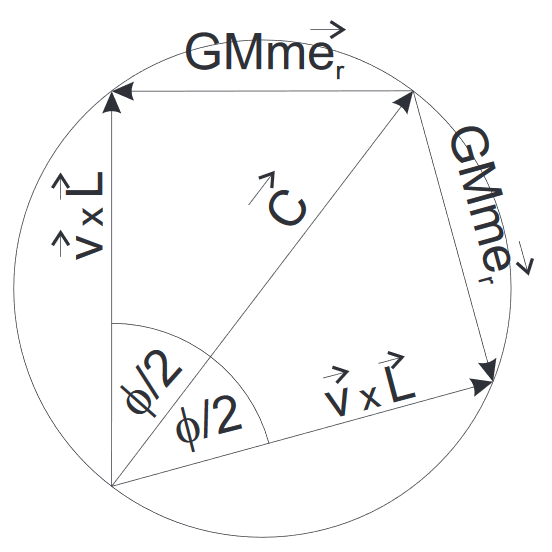
\includegraphics[width=0.35\linewidth]{Images/CM7.png}
\end{center}
Next, we need to calculate the angle $\phi$, but it is easier to first determine $\phi/2$ from the right triangle:
 $$\tan{\frac{\phi}{2}} = \frac{GmM}{vL} = \frac{GM}{v^2 b}, \ \ \   \tan{\phi} = \frac{\tan{\frac{\phi}{2}}+\tan{\frac{\phi}{2}}}{1-\tan^2{\frac{\phi}{2}}} = \frac{\tfrac{2GM}{v^2 b}}{1-{\left(\tfrac{GM}{v^2 b}\right)}^2},$$
 which gives us an answer of:
 $$\phi=\arctan\left(\dfrac{2GMv^2b}{v^4b^2-G^2M^2}\right).$$
\end{answer}
\vspace{-0.5cm}
\section{References}
\begin{biblist}
\bib{haloSE}{misc}{
    title={Are some Halo Orbits actually Stable?},    
    author={\href{https://space.stackexchange.com/users/12102/uhoh}{uhoh}},
    note={\href{https://space.stackexchange.com/q/15268}{https://space.stackexchange.com/q/15268} (version: 2020-04-11). The original source of the image no longer exists, but it is archived \href{https://web.archive.org/web/20160729215555/http://spacecraftforall.com/home}{here}},
    eprint={\href{https://space.stackexchange.com/q/15268}{https://space.stackexchange.com/q/15268}},
    organization={Space Exploration Stack Exchange}  
}
\bib{kaldakepler}{misc}{
    title={Kepleri seadused ja muu taevamehaanika},    
    author={Kree, Mihkel},
    date={2006},
    note={\href{https://www.ioc.ee/~kalda/ipho/kepler.pdf}{https://www.ioc.ee/~kalda/ipho/kepler.pdf}}
}
\end{biblist}
\end{document}